\documentclass[10pt, landscape]{article}
\usepackage[margin=0.25in]{geometry}
\usepackage{multicol}
\usepackage{amsmath, amssymb}
\usepackage{titlesec}
\usepackage{enumitem}
\usepackage{fancyhdr}
\usepackage{graphicx}
\usepackage{float}


% Cheatsheet styling
\titleformat{\section}{\large\bfseries}{}{0em}{}
\titlespacing{\section}{0pt}{*1}{*0.5}
\titleformat{\subsection}{\normalsize\bfseries}{}{0em}{}
\titlespacing{\subsection}{0pt}{*0.8}{*0.2}

\pagestyle{fancy}
\fancyhf{}
\rfoot{Page \thepage}
\setlength{\columnsep}{0.5cm}
\title{Stat 106 Cheatsheet}
\author{Cullen MacNeil}

\begin{document}
\begin{multicols}{3}

\begin{center}
    \textbf{Stat 106}
    \textbf{Cullen MacNeil}
\end{center}

\section{General Analytic \& Sports Metrics}

\subsection{Expected Points (EP)}
\begin{itemize}[noitemsep]
    \item Average points scored given a specific situation or state in a game.
    \item Calculated based on historical play-by-play data.
    \[ EP = \text{Shot Value} \times \text{Probability of Success} \]
    \item \textbf{Ex:} A 2-point shot with 53.6\% success chance: \(EP = 2 \times 0.536 = 1.072\)
\end{itemize}

\subsection{Expected Points Added (EPA)}
\begin{itemize}[noitemsep]
    \item Measure of value added by a play relative to expectation.
    \item Formula:
    \[ EPA = \text{Actual Points} - \text{EP} \]
    \item \textbf{Ex:} Player makes a 3pt shot with 35\% chance:
    \[ EP = 3 \times 0.35 = 1.05,\quad EPA = 3 - 1.05 = +1.95 \]
\end{itemize}

\subsection{Win Probability (WP) \& Win Probability Added (WPA)}
\begin{itemize}[noitemsep]
    \item \textbf{Win Probability (WP)}: Probability of winning given the current game state.
    \item \textbf{Win Probability Added (WPA)}: Change in WP from before to after a specific play.
    \item Formula:
    \[ WPA = WP_{\text{after}} - WP_{\text{before}} \]
    \item \textbf{Ex:} If WP rises from 0.03 to 0.05: \(WPA = 0.05 - 0.03 = +0.02\)
    \item High leverage situations (e.g., late-game) significantly affect WPA.
\end{itemize}

\section{Core Analytical Ideas}

\subsection{Stickiness, Leverage, Clutch-ness}
\begin{itemize}[noitemsep]
    \item \textbf{Stickiness}: Stability of performance metrics over time.
    \item \textbf{Leverage}: Situational importance; high-leverage moments significantly influence outcomes.
    \item \textbf{Clutch-ness}: Ability to perform well in high-leverage situations.
\end{itemize}

\subsection{Luck \& Mean Reversion}
\begin{itemize}[noitemsep]
    \item \textbf{Luck}: Random deviations from expected performance metrics.
    \item \textbf{Mean Reversion}: Tendency for extreme performance to return toward average levels over time.
\end{itemize}

\subsection{Shrinkage Estimates}
\begin{itemize}[noitemsep]
    \item Estimates adjusted towards a prior or mean to reduce variance.
    \item Useful for stabilizing performance estimates, particularly with limited data.
    \item Prevents overfitting and extreme predictions.
\end{itemize}

\section{Regression Models}

\subsection{Linear Regression}
\begin{itemize}[noitemsep]
    \item Model form: \( Y = \beta_0 + \beta_1 X + \epsilon \).
    \item Interpretation: Coefficient \(\beta_1\) is the average change in \(Y\) per unit change in \(X\).
    \item Assumptions: linearity, independence, homoscedasticity, normality.
\end{itemize}

\subsection{Logistic Regression}
\begin{itemize}[noitemsep]
    \item Used for binary outcomes; models log-odds of an event.
    \item Model form: \( \log\left(\frac{p}{1-p}\right) = \beta_0 + \beta_1 X \).
    \item Coefficients represent log-odds; \(e^{\beta}\) gives odds ratios.
\end{itemize}

\subsection{Linear vs Logistic}
\begin{itemize}[noitemsep]
    \item \textbf{Linear}: Continuous response variable.
    \item \textbf{Logistic}: Binary response variable.
    \item Choose based on outcome type (continuous vs. categorical).
\end{itemize}

\section{Transformations \& Interactions}

\subsection{Log Transformations}
\begin{itemize}[noitemsep]
    \item Used to stabilize variance or handle skewed predictors.
    \item Often applied to variables with exponential or multiplicative effects.
\end{itemize}

\subsection{Polynomial Transformations}
\begin{itemize}[noitemsep]
    \item Capture non-linear trends by including squared/cubic terms.
    \item Example: \( Y = \beta_0 + \beta_1X + \beta_2X^2 + \epsilon \).
    \item \(\epsilon\): Random error term; represents unexplained variation in \(Y\). Assumed to be normally distributed with mean 0 and constant variance.
\end{itemize}

\subsection{Interaction Effects}
\begin{itemize}[noitemsep]
    \item The effect of one variable depends on the level of another.
    \item Modeled with product terms: \( Y = \beta_0 + \beta_1X + \beta_2Z + \beta_3(XZ) + \epsilon \).
\end{itemize}

\vspace{0.5em}
\textbf{Log-Odds to Probability (Logistic Regression)}

\begin{itemize}[noitemsep]
    \item Model: \( \log\left(\frac{p}{1 - p}\right) = \beta_0 + \beta_1X \)
    \item The left-hand side is the \textbf{log-odds} of success.
    \item To convert to \textbf{odds}, exponentiate: 
    \[
    \text{odds} = e^{\beta_0 + \beta_1X}
    \]
    \item To convert odds to probability:
    \[
    p = \frac{\text{odds}}{1 + \text{odds}}
    \]
    \item \textbf{Example:} If log-odds = 0.8:
    \[
    \text{odds} = e^{0.8} \approx 2.23
    \]
    \[
    p = \frac{2.23}{1 + 2.23} \approx \frac{2.23}{3.23} \approx 0.69
    \]
\end{itemize}
\textbf{Note:} Odds \(= p / (1 - p)\) and probability \(= \text{odds} / (1 + \text{odds})\)



\section{Simulation \& Resampling}

\subsection{Bootstrapping}
\begin{itemize}[noitemsep]
    \item Repeated resampling from observed data to estimate sampling distribution.
    \item Useful for confidence intervals, bias estimation, and variance reduction.
\end{itemize}

\subsection{Permutation Testing}
\begin{itemize}[noitemsep]
    \item Hypothesis testing by reshuffling labels to determine significance.
    \item No assumptions about underlying distribution required.
\end{itemize}

\section{Rating \& Ranking Systems}

\subsection{Bradley-Terry Models}
\begin{itemize}[noitemsep]
    \item Assigns each team a latent strength \( \lambda_i \).
    \item Win probability: 
    \[
    P(A \text{ beats } B) = \frac{1}{1 + e^{\lambda_B - \lambda_A}}
    \]
    \item Fit via logistic regression on match results.
    \item Ties not natively handled — average models treating ties as wins and losses.
\end{itemize}

\textbf{Quantitative BT Extension:}
\begin{itemize}[noitemsep]
    \item Predicts numeric outcomes (e.g., point differential) instead of binary wins.
\end{itemize}

\vspace{0.3em}
\subsection{Elo Models}
\begin{itemize}[noitemsep]
    \item Dynamic update system — ratings evolve after each match.
    \item Win probability:
    \[
    P(\text{A beats B}) = \frac{1}{1 + 10^{(R_B - R_A)/400}}
    \]
    \item Rating update:
    \[
    R_{\text{new}} = R_{\text{old}} + k(\text{Outcome} - \text{Expected})
    \]
    \item Outcomes: 1 = win, 0.5 = draw, 0 = loss. \(k\) = sensitivity.
\end{itemize}

\textbf{Elo Example:}
\begin{itemize}[noitemsep]
    \item \(R_A = 1500\), \(R_B = 1600\), \(k = 50\), A wins.
    \item \(P = \frac{1}{1 + 10^{(1600-1500)/400}} \approx 0.36\)
    \item \(R_A = 1500 + 50(1 - 0.36) = 1532\), \(R_B = 1600 - 50(0.64) = 1568\)
\end{itemize}

\vspace{0.3em}
\textbf{Bradley-Terry vs. Elo}
\begin{itemize}[noitemsep]
    \item \textbf{BT:} Static strengths from full dataset, fitted once.
    \item \textbf{Elo:} Dynamic updates over time, match-by-match.
    \item \textbf{BT:} Assumes independence; \textbf{Elo:} incorporates time ordering.
\end{itemize}

\subsection{KenPom Efficiency}
\begin{itemize}[noitemsep]
    \item Basketball-specific metrics evaluating team efficiency.
    \item Offensive and defensive ratings adjusted for opponent strength and pace.
    \item Higher efficiency indicates stronger overall performance.
\end{itemize}


\section{Predictive Modeling \& Validation}

\subsection{Train-Test-Validation Split}
\begin{itemize}[noitemsep]
    \item Data partitioned into subsets:
    \begin{itemize}[noitemsep]
        \item \textbf{Training}: Model fitting.
        \item \textbf{Validation}: Model selection and tuning.
        \item \textbf{Test}: Evaluate out-of-sample predictive performance.
    \end{itemize}
\end{itemize}

\subsection{Cross-Validation}
\begin{itemize}[noitemsep]
    \item Technique to assess model predictive performance.
    \item Data repeatedly split into training and validation subsets.
    \item Commonly used form: k-fold CV, data split into k subsets.
\end{itemize}

\subsection{Prediction, Overfitting, Complexity}
\begin{itemize}[noitemsep]
    \item \textbf{Overfitting}: Model captures noise, poor generalization.
    \item Balance complexity (number of parameters) vs. prediction accuracy.
    \item Cross-validation helps identify appropriate model complexity.
\end{itemize}

\section{Model Selection \& Regularization}

\subsection{Model Selection: AIC \& BIC}
\begin{itemize}[noitemsep]
    \item Used in sequential variable selection to balance fit and complexity.
    \item \textbf{AIC:} 
    \[
    AIC = 2(p+1) - 2\ln(\hat{L})
    \]
    \item \textbf{BIC:} 
    \[
    BIC = 2\ln(n) - 2\ln(\hat{L})
    \]
    \item Both penalize model complexity; BIC does so more heavily.
    \item AIC → better prediction focus; BIC → better for finding simpler models.
\end{itemize}

\subsection*{Penalized Regression Overview}
\begin{itemize}[noitemsep]
    \item Penalized regression minimizes an objective of the form:
    \[
    \text{SSE} + \lambda \sum_j \text{Penalty}(\beta_j)
    \]
    \item \(\lambda\): regularization strength (chosen via cross-validation).
    \item Predictors typically standardized before fitting.
\end{itemize}

\subsection{Ridge Regression}
\begin{itemize}[noitemsep]
    \item Minimizes: \( \text{SSE} + \lambda \sum_j \beta_j^2 \)
    \item Shrinks coefficients smoothly toward 0 (none exactly 0).
    \item Keeps all predictors; useful with many small effects.
    \item Has a closed-form solution.
\end{itemize}

\subsection{LASSO Regression}
\begin{itemize}[noitemsep]
    \item Minimizes: \( \text{SSE} + \lambda \sum_j |\beta_j| \)
    \item Shrinks some coefficients exactly to 0 → performs variable selection.
    \item Sparse, interpretable models; no closed-form solution.
\end{itemize}


\vspace{0.3em}
\textbf{Choosing Between Methods}
\begin{itemize}[noitemsep]
    \item \textbf{Sequential selection:} Good with few strong predictors.
    \item \textbf{Ridge:} Good with many weak/moderate predictors.
    \item \textbf{LASSO:} Best with mix of useful and useless predictors.
    \item Compare models using validation/test MSE, not just training fit.
\end{itemize}

\textbf{Penalty Comparison Table:}

{\scriptsize
\begin{tabular}{|l|c|c|c|}
\hline
\textbf{Method} & \textbf{Penalty} & \textbf{Zero Coefs?} & \textbf{Closed Form?} \\\hline
OLS & -- & No & Yes \\
Ridge & \( \lambda \sum \beta_j^2 \) & No & Yes \\
LASSO & \( \lambda \sum |\beta_j| \) & Yes & No \\\hline
\end{tabular}
}



\section{Advanced Predictive Techniques}

\subsection{Random Forests}
\begin{itemize}[noitemsep]
    \item Ensemble of decision trees built on bootstrapped samples.
    \item Reduces variance and improves prediction by averaging outcomes.
    \item Each split considers random subset of predictors.
\end{itemize}

\subsection{Hyperparameter Tuning}
\begin{itemize}[noitemsep]
    \item Process of optimizing model parameters not learned from data.
    \item Common methods: Grid Search, Random Search, Cross-Validation.
    \item Helps prevent overfitting and improves predictive performance.
\end{itemize}

\section{Additional Quick Reference}

\subsection{Regression Assumptions}
\textbf{OLS Linear Regression}:
\begin{itemize}[noitemsep]
    \item OLS = Ordinary Least Squares
    \item Linearity, independence, homoscedasticity, normality of residuals.
\end{itemize}

\textbf{Logistic Regression}:
\begin{itemize}[noitemsep]
    \item Independence, linearity in logit scale.
\end{itemize}

\subsection{Important Metrics \& Formulas}

\textbf{Pythagorean Wins}:
\[
\text{Wins} = \frac{\text{Runs Scored}^2}{\text{Runs Scored}^2 + \text{Runs Against}^2} \times \text{Games} 
\]

\textbf{Confidence Interval (mean)}:
\[
\bar{x} \pm t^*\frac{s}{\sqrt{n}}
\]

\textbf{Z-Test Statistic}:
\[
Z = \frac{\bar{x} - \mu_0}{\sigma/\sqrt{n}}
\]

\subsection*{Conditional Distribution of $Y \mid X$ (Regression)}

\begin{itemize}[noitemsep]
    \item In linear regression:  
    \[
    Y \mid X \sim N(\mu = \beta_0 + \beta_1 X, \sigma^2)
    \]
    
    \item Use this to estimate probabilities of outcomes:
    \begin{align*}
    P(Y > a \mid X = x) 
    &= P\left(Z > \frac{a - \mu}{\sigma}\right)
    \end{align*}
    where \( \mu = \beta_0 + \beta_1 x \)

    \item \textit{\textbf{Note:}} \( a \) is the outcome threshold of interest  
    (e.g., \( a = 0 \) if you're asking the probability that a team wins a game).
\end{itemize}

\textbf{Example:}
\[
\beta_0 = 7.135, \quad 
\beta_1 = 3.224, \quad 
\hat{\sigma} = 14.46
\]

\begin{align*}
P(Y > 0 \mid X = 1) 
&= P\left(Z > \frac{0 - (7.135 + 3.224 \cdot 1)}{14.46} \right) \\
&= P\left(Z > \frac{-10.36}{14.46} \right) = P(Z > -0.72) \\
&= P(Z < 0.72) \approx 0.7642
\end{align*}



\subsection{Model Interpretation}
\begin{itemize}[noitemsep]
    \item Linear regression coefficient: change in \(Y\) per unit change in \(X\).
    \item Logistic regression coefficient: log-odds, \(e^\beta\) for odds ratio.
    \item Adjusted \(R^2\): accounts for number of predictors.
\end{itemize}

\section{Coefficient Plot Comparison}

{\scriptsize
\begin{tabular}{|l|l|}
\hline
\textbf{Model} & \textbf{Path Summary} \\\hline
\textbf{Seq. Select} & Jumps at steps; adds/removes variables. \\\hline
\textbf{Ridge} & Coefs shrink smoothly; asymptote to 0. \\\hline
\textbf{LASSO} & Some coefs shrink exactly to 0 (sparse model). \\\hline
\end{tabular}
}

\vspace{0.5em}
\begin{figure}[H]
\centering
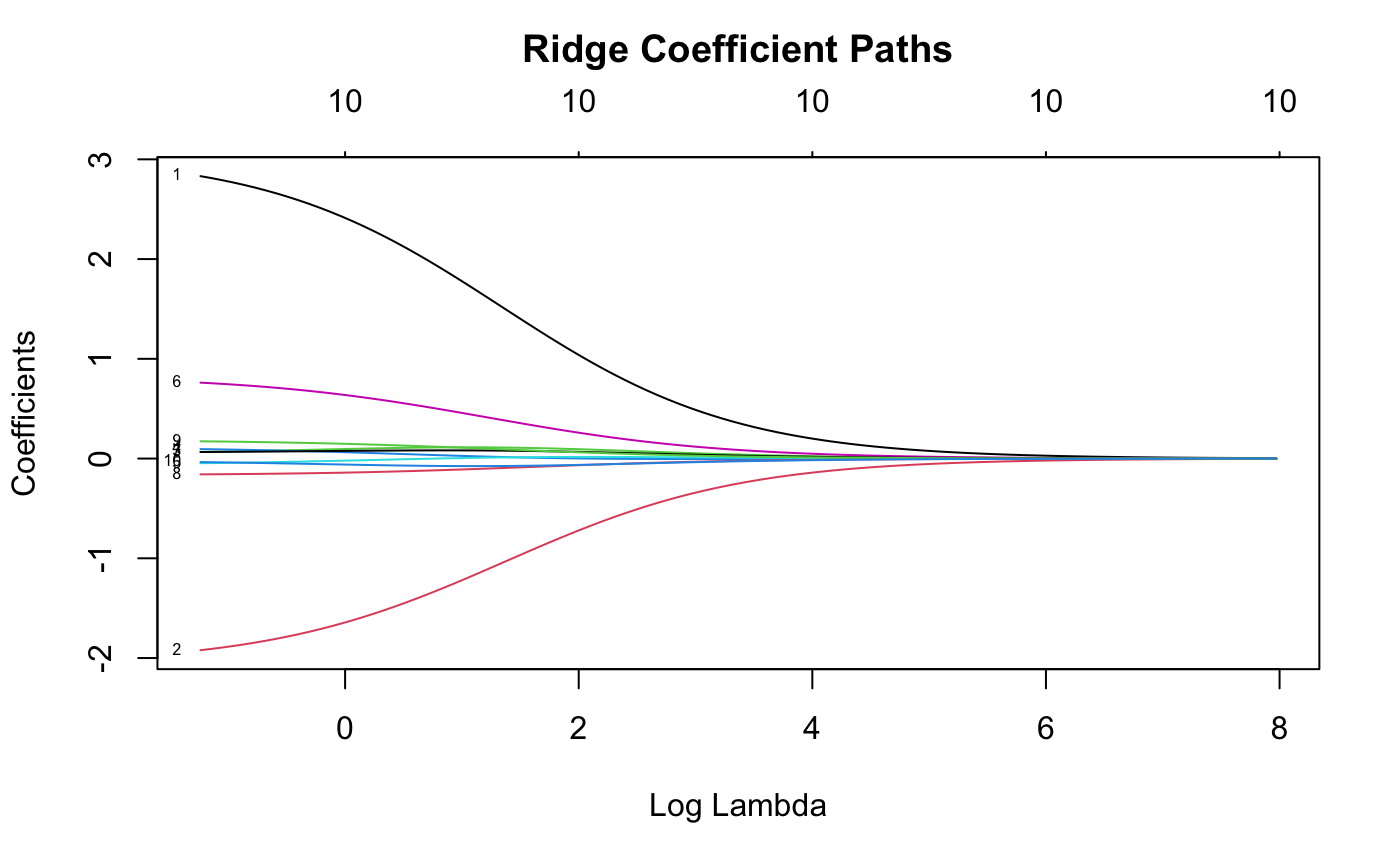
\includegraphics[width=0.95\linewidth]{Ridge coeff path.png}
\vspace{-0.5em}
\caption*{\scriptsize \textbf{Ridge Coeff Paths:} Coefficients shrink smoothly but do not hit zero.}
\end{figure}

\begin{figure}[H]
\centering
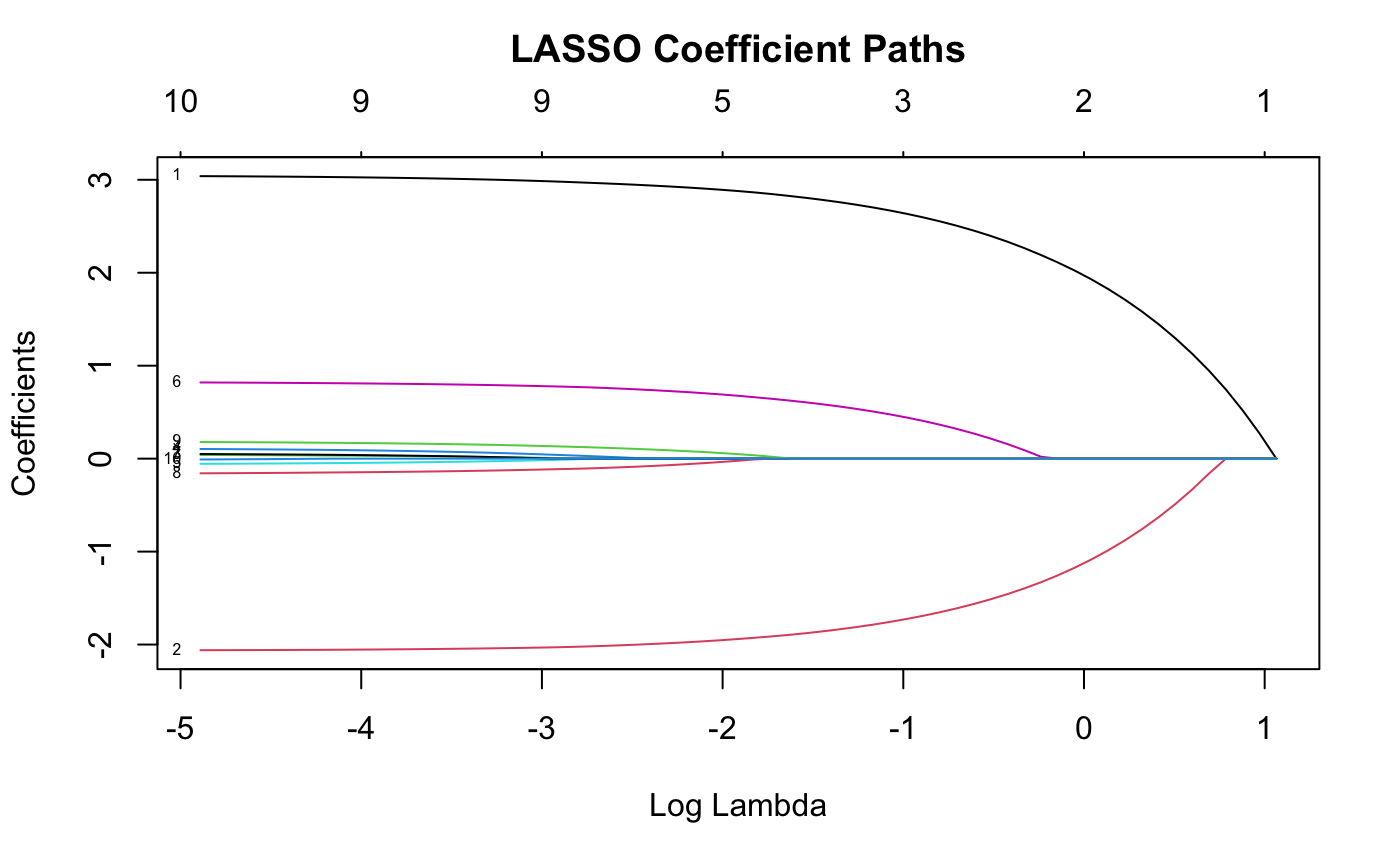
\includegraphics[width=0.95\linewidth]{Lasso Coef path.png}
\vspace{-0.5em}
\caption*{\scriptsize \textbf{LASSO Coeff Paths:} Some coefficients shrink exactly to 0 (variable selection).}
\end{figure}

\begin{figure}[H]
\centering
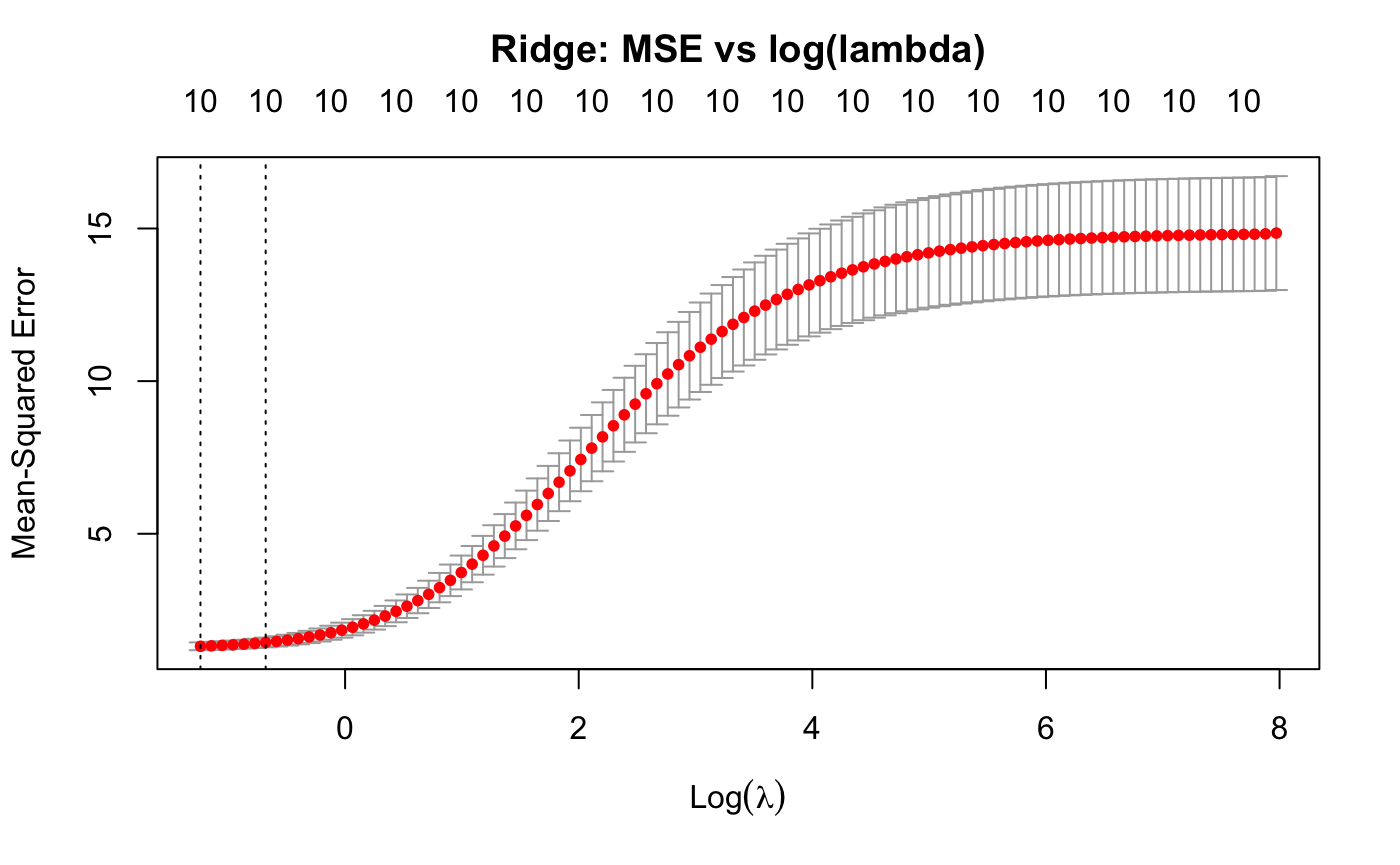
\includegraphics[width=0.95\linewidth]{Ridge MSE.png}
\vspace{-0.5em}
\caption*{\scriptsize \textbf{Ridge CV:} MSE curve across \(\log(\lambda)\); optimal \(\lambda\) balances bias-variance.}
\end{figure}

\begin{figure}[H]
\centering
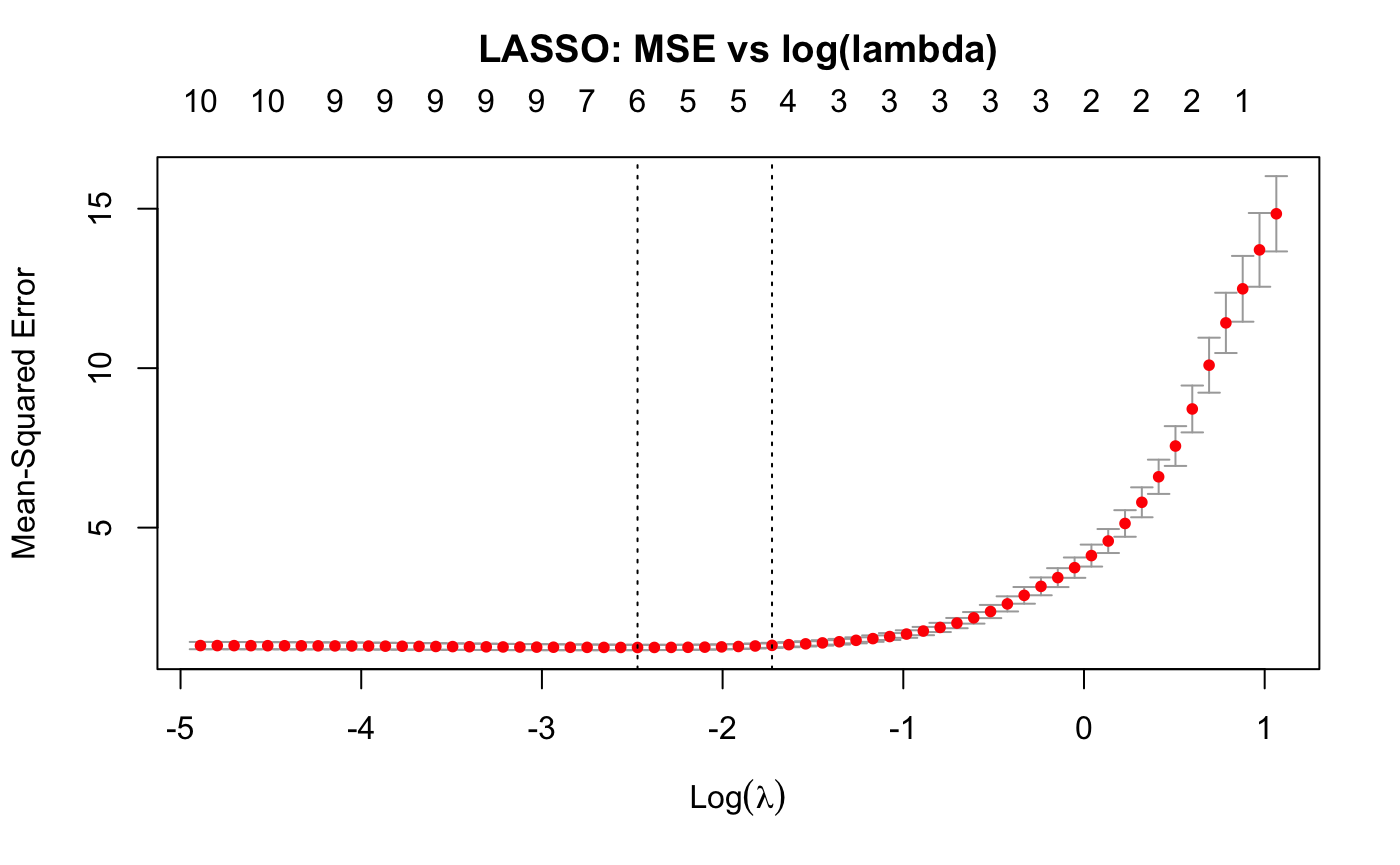
\includegraphics[width=0.95\linewidth]{Lasso MSE.png}
\vspace{-0.5em}
\caption*{\scriptsize \textbf{LASSO CV:} MSE minimized where most unimportant coefficients are shrunk to 0.}
\end{figure}


\end{multicols}
\end{document}
